\newpage
\section{Hydrodynamik}

\subsection{Kontinuitätsgleichung}				%Kontinuitätsgleichung
\begin{table}[h!]
	\begin{tabular}{ | m{6cm} | m{6cm} | m{6cm} | }
		\hline
		Abbildung & Formeln & Einheiten \\ \hline
		\midrule
		\begin{minipage}{.3\textwidth}
			\includegraphics[width=6.0cm]{Figures/kontinuitaet}
		\end{minipage}
		&
		%\begin{minipage}[t]{5cm}
		\begin{itemize}
			\item $A_{1}*v_{1}=A_{2}*v_{2}$			
		\end{itemize}
		%\end{minipage}
		& 
		%\begin{minipage}{5cm}
		\begin{itemize}
			\item $A_{1},A_{2}=[m^2]$
			\item $v_{1},v_{2}=[\frac{m}{s}]$	
		\end{itemize}
		%\end{minipage}
		\\ \hline
	\end{tabular}
\end{table}

\subsection{Bernoulli-Gleichung}				%Bernoulli-Gleichung
\begin{table}[h!]
	\begin{tabular}{ | m{6cm} | m{8cm} | m{4cm} | }
		\hline
		Abbildung & Formeln & Einheiten \\ \hline
		\midrule
		\begin{minipage}{.3\textwidth}
			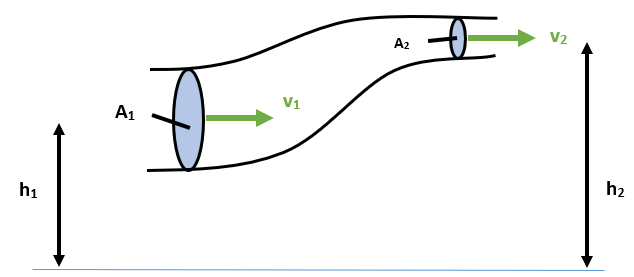
\includegraphics[width=6.2cm]{Figures/bernoulli}
		\end{minipage}
		&
		%\begin{minipage}[t]{5cm}
		\begin{itemize}
			\item$p_{1}+\rho*\dfrac{v_{1}^2}{2}+\rho*g*h_{1}=p_{2}+\rho*\dfrac{v_{2}^2}{2}+\rho*g*h_{2}$	\item$p_{1,2}=$ Statischer Druck
			\item$\rho*\dfrac{v_{1,2}^2}{2}=$ Dynamischer Druck
			\item$\rho*g*h_{1,2}=$ Schweredruck	
		\end{itemize}
		%\end{minipage}
		& 
		%\begin{minipage}{5cm}
		\begin{itemize}
			\item $p_{1,2}=[\frac{N}{m^2}]=Pa$
			\item $v_{1,2}=[\frac{m}{s}]$	
			\item $\rho=[\frac{kg}{m^3}]$	
		\end{itemize}
		%\end{minipage}
		\\ \hline
	\end{tabular}
\end{table}

\subsection{Formel von Stokes - Kugelfallviskosimeter}				%Formel von Stokes - Kugelfallviskosimeter
\begin{table}[h!]
	\begin{tabular}{ | m{4cm} | m{10cm} | m{4cm} | }
		\hline
		Abbildung & Formeln & Einheiten \\ \hline
		\midrule
		\begin{minipage}{.3\textwidth}
			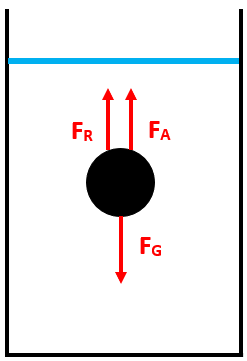
\includegraphics[width=4.2cm]{Figures/Stokes}
		\end{minipage}
		&
		%\begin{minipage}[t]{5cm}
		\begin{itemize}
			\item Im Gleichgewicht: $F_{G}=F_{A}+F_{R}$	
			\item $F_{Gewicht}=\frac{4}{3}*\pi *r^{3}* \rho_{Koerper} *g=m*g$	 
			\item $F_{Auftrieb}=\frac{4}{3}*\pi *r^{3}* \rho_{Fluessigkeit} *g=m*g$
			\item $F_{Reib}=6*\pi *r^{3}* \eta*r*v$	
			\item $\eta=$Viskosität$=\dfrac{2*r^{2}*g*(\rho_{K}-\rho_{F})}{9*v}$
		\end{itemize}
		%\end{minipage}
		& 
		%\begin{minipage}{5cm}
		\begin{itemize}
			\item $F_{G},F_{A},F_{R}=[N]$
			\item $r=[m]$	
			\item $\rho_{K},\rho_{F},=[\frac{kg}{m^3}]$	
			\item $g=[\frac{m}{s^{2}}]$
			\item $m=[kg]$
			\item $\eta=[\frac{N*s}{m^{2}}]$
		\end{itemize}
		%\end{minipage}
		\\ \hline
	\end{tabular}
\end{table}

\newpage

\subsection{Laminare Rohrströmung}				%Laminare Rohrströmung
\begin{table}[h!]
	\begin{tabular}{ | m{7cm} | m{7cm} | m{4cm} | }
		\hline
		Abbildung & Formeln & Einheiten \\ \hline
		\midrule
		\begin{minipage}{.3\textwidth}
			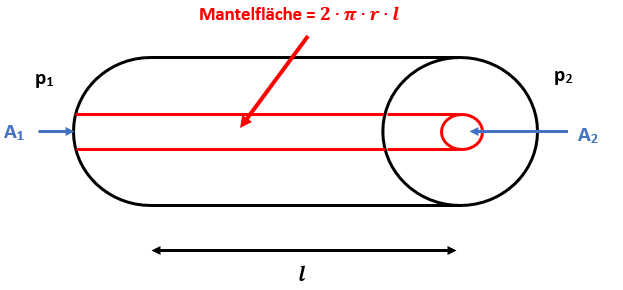
\includegraphics[width=7.2cm]{Figures/laminar}
		\end{minipage}
		&
		%\begin{minipage}[t]{5cm}
		\begin{itemize}
			\item $F_{Reib}=F_{Druck1}-F_{Druck2}$	
			\item $\tau=\pi*r^{2}*(p_{1}-p_{2})+2*\pi*r*l*\eta*\frac{dv}{dr}$	
			\item $\tau=Schubspannung$

		\end{itemize}
		%\end{minipage}
		& 
		%\begin{minipage}{5cm}
		\begin{itemize}
			\item $\tau,p_{1},p_{2}=[Pa]$
			\item $r,l=[m]$
			\item $F=[N]$
			\item $\eta=$ Viskosität $=[\dfrac{kg}{m*s}]=[Pa*s]$
		\end{itemize}
		%\end{minipage}
		\\ \hline
	\end{tabular}
\end{table}

\subsection{Gesetz von Hagen Poiseuille}				%Gesetz von Hagen Poiseuille
\begin{table}[h!]
	\begin{tabular}{ | m{9cm} | m{9cm}  | }
		\hline
		Formeln & Einheiten \\ \hline
		\midrule
		%\begin{minipage}[t]{5cm}
		\begin{itemize}
			\item \.{V}$=\dfrac{V}{t}=\dfrac{\pi*\Delta p*r^{4}}{8*\eta*l}=\dfrac{\pi*(p_{2}-p_{1})*r^{4}}{8*\eta*l} $	
		\end{itemize}
		%\end{minipage}
		&
		%\begin{minipage}{5cm}
		\begin{itemize}
			\item $\Delta p,p_{2},p_{1}= [\frac{N}{m^{2}}]=[Pa]$
			\item \.{V}$=[m^3]$
			\item $P=[W]$
			\item $F=[N]$
			\item $A=[m^{2}]$
			\item $s=[m]$
			\item $\eta=$ Viskosität $=[\dfrac{kg}{m*s}]=[Pa*s]$
		\end{itemize}
		%\end{minipage}
		\\ \hline
	\end{tabular}
\end{table}

\subsection{Pumpenleistung}				%Pumpenleistung
\begin{table}[h!]
	\begin{tabular}{ | m{9cm} | m{9cm}  | }
		\hline
		Formeln & Einheiten \\ \hline
		\midrule
		%\begin{minipage}[t]{5cm}
		\begin{itemize}
			\item $P=\dfrac{W}{t*\eta}=\dfrac{F*s}{t*\eta}=\dfrac{p*A*s}{t*\eta}=\dfrac{p*V}{t*\eta}$	
		\end{itemize}
		%\end{minipage}
		&
		%\begin{minipage}{5cm}
		\begin{itemize}
			\item $p= [\frac{N}{m^{2}}]=Pa$
			\item $V=[m^3]$
			\item $P=[W]$
			\item $F=[N]$
			\item $A=[m^{2}]$
			\item $s=[m]$
			\item $\eta=$ Wirkungsgrad $=[1]$
		\end{itemize}
		%\end{minipage}
		\\ \hline
	\end{tabular}
\end{table}

\newpage

\subsection{Reynolds-Zahl}				%Reynolds-Zahl
\begin{table}[h!]
	\begin{tabular}{ | m{9cm} | m{9cm}  | }
		\hline
		Formeln & Einheiten \\ \hline
		\midrule
		%\begin{minipage}[t]{5cm}
		\begin{itemize}
			\item $Reynoldszahl=Re=\dfrac{\rho*v*d}{\eta}=\dfrac{\rho*\dot{V}*4}{d*\pi*\eta}$	
			\item $v=\dfrac{\dot{V}}{A}$
			\item $Re>2320\Rightarrow$ Bei Rohrströmung Turbulenz
			\item $Re<2320\Rightarrow$ Keine Turbulenz
		\end{itemize}
		%\end{minipage}
		&
		%\begin{minipage}{5cm}
		\begin{itemize}
			\item $\rho=[\dfrac{kg}{m^3}]$
			\item $\eta=$ Viskosität $=[\dfrac{kg}{m*s}]=[Pa*s]$
			\item $v=[\frac{m}{s^2}]$
			\item $d=[m]$
			\item $A=[m^2]$
			\item $\dot{V}=[\frac{m^3}{s}]$
			
		\end{itemize}
		%\end{minipage}
		\\ \hline
	\end{tabular}
\end{table}
